\section{Visualizing undirected comparative distributions}\label{sec:ComparativeUndirected}

In order to compare two languages in terms of the way a given
functional domain is structured, a common procedure is to use a
semantic or functional criterion as a third of comparison, and then
determine the way the semantic space in question is mapped to linguistic expressions \citep{Gast2012}. In our case, this means that
we use the functional annotations as a \textit{tertium comparationis},
and we locate the expressions from different languages relative to
these annotations.

In Sect. \ref{sec:LanguageSpecific} we used four methods to visualize
form-function mappings in specific languages: CA -- with and without
stacked tables -- and MCA -- with and without supplementary variables. In this
section we focus on only one of these methods, MCA with
supplementary variables. The advantage of an MCA over a CA (with
stacked tables) is that it allows us a per-item analysis, as each
observation, and not just the variables, are located in low-dimensional space. The advantage of an MCA with supplementary variables is that it
creates a coordinate system that is independent of the specific expressions
used in a language, so we can (comparatively) locate expressions from
different languages in that system. Put differently, the coordinate system is
constituted by the distributional variables, functioning as the
\textit{tertium comparationis}, while the expressions are the  \textit{comparanda}.

An MCA with `IP-adverbial' as a supplementary variable is shown for
original occurrences of \textit{gleich}, \textit{sofort},
\textit{immédiatement} and \textit{tout de suite} in Figure
\ref{fig:MCADeFrSup}, relative to four distributional variables
(\textsc{intentionality}, \textsc{Agent}, \textsc{Illocutionary force}
and \textsc{Reference point}).


\begin{figure}
  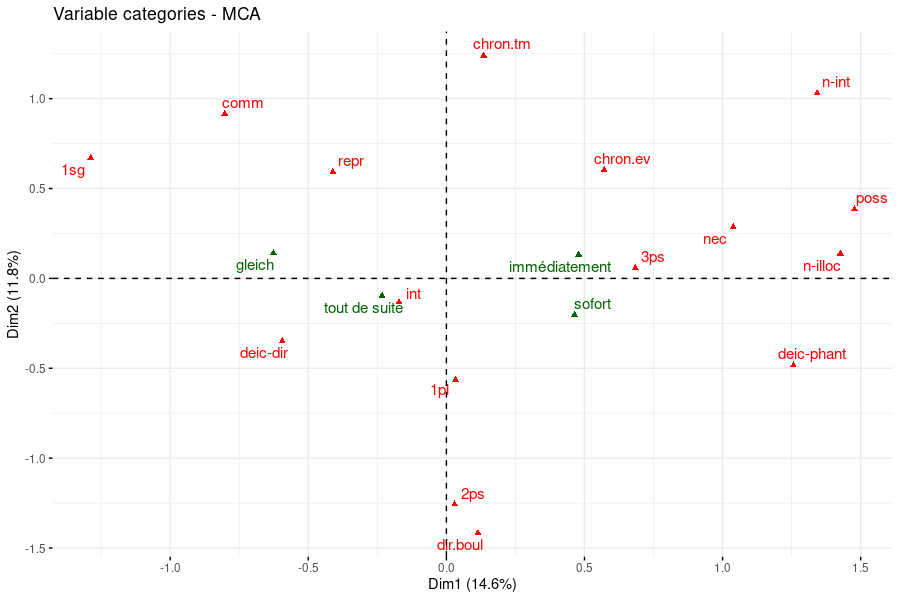
\includegraphics[width=\linewidth]{figures/MCA-sup-de-fr.png}
  \cprotect\caption{MCA with IP-adverbial as supplementary variable
    (German and originals), relative to the variables
    `intentionality', `agent', `illocutionary force' and `reference
    point'. The CA was created with the package \verb+FactoMineR+ for
    \verb+R+ \citep{FactoMineR-package}, for the visualization we used
    the package \verb+factoextra+ \citep{factoextra-package}. The
    adjusted percentages of explained inertia as returned by the
    package \verb+ca+ for \verb+R+ \citep{ca-package} are 48.5\% (Axis
    1) and 15.0\% (Axis 2).}
  \label{fig:MCADeFrSup}
\end{figure}

Though no doubt quite informative, Figure \ref{fig:MCADeFrSup} is
hard to read. A general observation that stands out is that
the four adverbials are located in different quadrants of the
plot. Another relevant observation is that \textit{tout de suite} is
considerably closer to the centre than the other adverbials, which
suggests a less specialized distribution for this adverbial.

One way of simplifying a multivariate distribution as shown in Figure
\ref{fig:MCADeFrSup} is to apply clustering. As an MCA locates every
single observation in the new space that it creates, we can
identify clusters of similar observations. We used PAM (partitioning
around medoids) clustering for this purpose, which identifies clusters
on the basis of distances between observations -- as the name
suggests, around a medoid, i.e., a (representative) observation in the
centre of the cluster. \footnote{We used the package \verb+cluster+
  for \verb+R+, cf. \citet{cluster-package}. We validated the
  clustering solution using the silhouette method (see the package
  documentation for more information).} Clusters with 3 or 6 medoids
were chosen because the average silhouette scores showed visible leaps
at these points (in comparison to solutions with 2 and 5 clusters; see
Figure \ref{fig:Silhouette}, Sect. \ref{sec:AppComparativeUndirected},
in the Appendix). The location of clusters of individual sentences in
the coordinate system defined by the MCA is visualized in Figure
\ref{fig:MCACluster}.
%
The annotations for the medoid observations of the clusters are shown
in Table \ref{tab:Medoids}. The corresponding examples are provided in
\bv{ClusterEx1}--\bv{ClusterEx3}. 

\pagebreak

\begin{table}[H]
  \centering
  \scriptsize
    \begin{tabular}[h]{llllll|llllll}
    ID  & agent &int &mod   &   ref & cl & ID  & agent &int &mod   &   ref & cl \\\hline
    448   &1sg &int     &repr &deic-dir & 1 & 448   &1sg   &int     &repr   &deic-dir  &     1 \\
    16    &3ps &int     &repr &chron.ev & 2 & 41    &3ps   &int     &repr   &deic-dir  &     2 \\
    443   &3ps &int &dir.boul &deic-dir & 3 & 443  & 3ps   &int &dir.boul   &deic-dir  &     3 \\
    &   &&&&&441   &3ps   &int   &  repr &  chron.ev &      4\\
    &   &&&&&455   &3ps   &int &dir.boul &  chron.ev  &     5\\
    &   &&&&&280   &3ps &n-int  &   repr &deic-phant  &     6\\
  \end{tabular}
  \caption{Medoid observations for cluster solutions with 3 (left) and 6 (right) clusters}
  \label{tab:Medoids}
\end{table}

\begin{exe}
  \ex\label{ClusterEx1}
  \begin{xlist}
    \ex Je lui donne bien volontiers tout de suite la parole. (original)
    \ex Ich erteile ihm daher gern sogleich das Wort.
    \ex I am very happy to give you the floor now.
  \end{xlist}
  \ex\label{ClusterEx2}
  \begin{xlist}
    \ex C'est une expérience amère, lorsque l'on fait des propositions
    de réforme, de constater que d'autres les bloquent constamment
    avec des référence à autre chose.
    \ex Ich finde es bitter, wenn
    man Reformvorschläge macht, dass die gleich immer so abgeblockt
    und mit etwas anderem in Bezug gebracht werden. (original)
    \ex It is a bitter experience, when one makes reform proposals, to find
    that others are constantly blocking them with reference to
    something else.
  \end{xlist}
  \ex\label{ClusterEx3}
  \begin{xlist}
    \ex Il faut mettre ce régime sous tutelle internationale et il faut le faire tout de suite!
    \ex Dieses Regime muß unter internationale Aufsicht gestellt werden, und zwar sofort! (original)
    \ex This regime needs to be placed under international supervision, and this should be done straight away! 
  \end{xlist}
\end{exe}
%
In the French and German versions of the medoid of Cluster 1
(cf. \bv{ClusterEx1}) we find \textit{tout de suite} and
\textit{sogleich}, arguably a stylistic variant of
\textit{gleich}. The medoid of Cluster 2 (cf. \bv{ClusterEx2}) also
has \textit{gleich} in German but no expression in French -- a not
uncommon situation. The medoid of Cluster 3 (cf. \bv{ClusterEx3}) has
\textit{sofort} in German and \textit{tout de suite} in French. This
illustrates that the clusters are not actually constituted by German
or French expressions. They represent characteristic utterance types
defined by the distributional variables: (i) a (typically deictic)
declaration of future action by the speaker (Cluster 1); (ii) a
(typically chronological) statement about a third person (Cluster 2);
and (iii) a call for action (Cluster 3).

\begin{figure}[t]
  \centering
  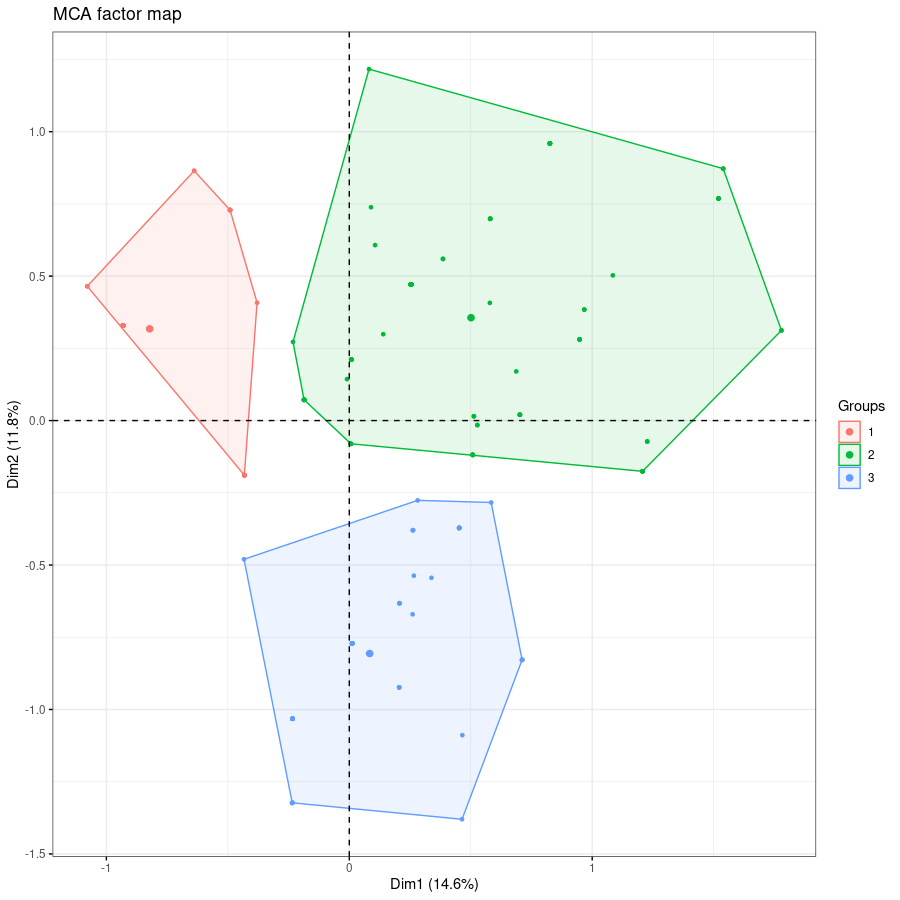
\includegraphics[width=0.45\linewidth]{figures/cluster-low.png}
  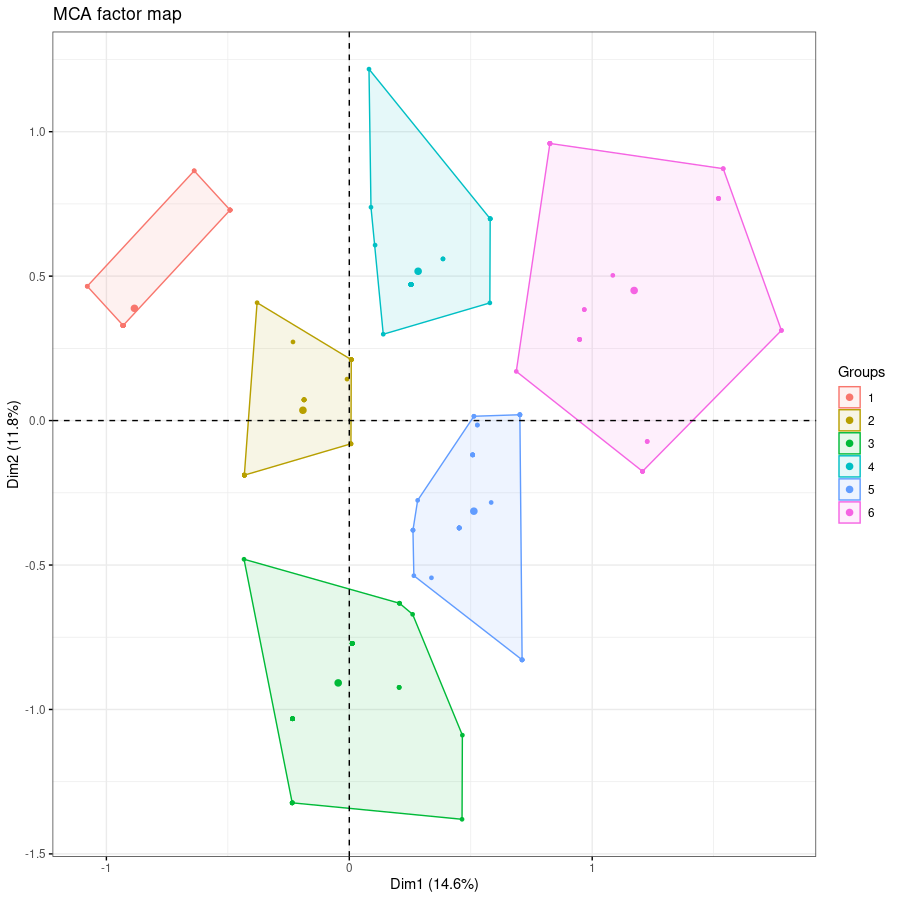
\includegraphics[width=0.45\linewidth]{figures/cluster-high.png}
  \cprotect\caption{Clusters based on MCA-coordinates and
    PAM-clustering with three (left) and six (right)
    clusters, using the package \verb+cluster+ for \verb+R+
    \citep{cluster-package}. The plots were generated with the package
    \verb+factoextra+ for R \citep{factoextra-package}.}
  \label{fig:MCACluster}
\end{figure}
%
In order to understand associations between clusters (major use types)
and \ipadv s we can cross-tabulate the \ipadv s with the clusters of
the two cluster solutions. Relevant mosaic plots are shown in Figure
\ref{fig:MosaicClusters}. Both plots suggest a positive association of
Cluster 1 with \textit{gleich}. The plot with six clusters moreover
shows positive associations between \textit{immédiatement} and Cluster
6, and between \textit{sofort} and Cluster 5. Another important
observation is that \textit{tout de suite} does not show an
association with any of the clusters. This confirms our impression
that it is the most generic/least specialized expression of the \ipadv
s under investigation.

\begin{figure}[b]
  \centering
  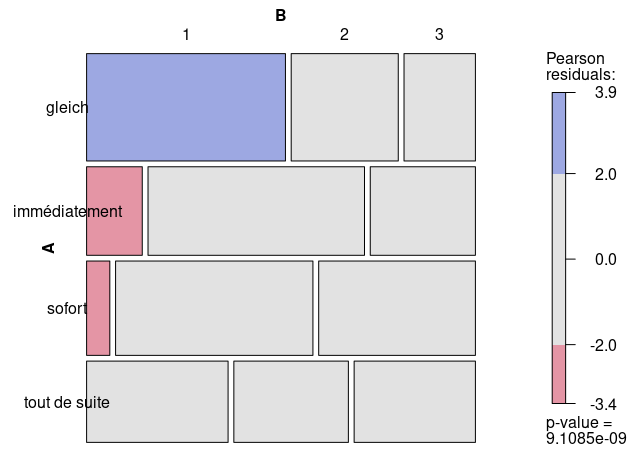
\includegraphics[width=0.45\linewidth]{figures/mosaic-cluster-low.png}
  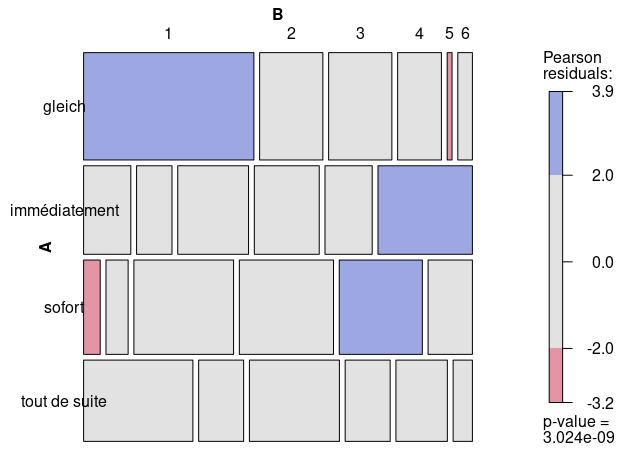
\includegraphics[width=0.45\linewidth]{figures/mosaic-cluster-high.png}
  \cprotect\caption{Mosaic plots for cross-tabulations of German and French
    \ipadv s with clusters, for cluster solutions with three (left) and six (right)
    clusters. The plots were generated with the package \verb+vcd+ for
    \verb+R+ \citep{vcd-package}.}
  \label{fig:MosaicClusters}
\end{figure}

The visualization methods that can be used for undirected comparative
data are thus essentially the same as those that were discussed for
language-specific data. 
%, and all of the other methods that were discussed under `proportional visualizations' are of course also in principle available.
What distinguishes comparative data from language-specific data is primarily the use of
an appropriate \textit{tertium comparationis}. This is a conceptual
rather than technical matter. Note also that -- as was pointed out
above -- in undirected comparative (e.g., contrastive) studies, it is
always helpful to visualize language-specific distributions as
well. For example, it is of course conceivable for context variables
to behave differently (e.g., in their clustering behaviour) across
languages. Such differences can best be identified by inspecting and
comparing language-specific distributions, potentially identifying
hypotheses that can be tested with inferential statistics.




%%% Local Variables:
%%% mode: latex
%%% TeX-master: "main"
%%% End:
